\documentclass{bioinfo}
\copyrightyear{2016} \pubyear{2016}

\access{Advance Access Publication Date: Day Month Year}
\appnotes{Original Paper}

\begin{document}
\firstpage{1}

\subtitle{Systems Biology}

\title[One model to rule them all]{One model to rule them all}
\author[Steiert \textit{et~al}.]{Bernhard Steiert\,$^{\text{\sfb 1,}*}$, Jens Timmer\,$^{\text{\sfb 1,2}}$ and Clemens Kreutz\,$^{\text{\sfb 1}}$}
\address{$^{\text{\sf 1}}$Institute of Physics, University of Freiburg, Germany and \\
$^{\text{\sf 2}}$BIOSS Centre for Biological Signalling Studies, University of Freiburg, Germany.}

\corresp{$^\ast$To whom correspondence should be addressed.}

\history{Received on XXXXX; revised on XXXXX; accepted on XXXXX}

\editor{Associate Editor: XXXXXXX}
% This abstract is more or less a placeholder and needs to be rewritten.
\abstract{\textbf{Motivation:}
A major goal in systems biology is to reveal potential drug targets for cancer therapy.
Signaling pathways triggering cell-fate decisions are often altered in cancer resulting in uncontrolled proliferation and tumor growth.
However, addressing cancer-specific alterations experimentally by investigating each node in the signaling network one after the other is difficult or even not possible at all.\\
\textbf{Results:} Here, we combined quantitative time-resolved data from different cell lines with non-linear modeling under L1 regularization, which is capable of detecting cell-type specific parameters.
To adapt the least-squares numerical optimization routine to L1 regularization, sub-gradient strategies as well as truncation of proposed optimization steps were implemented.
Likelihood-ratio test is used to determine the optimal penalization strength resulting in a sparse solution in terms of a minimal number of cell-type specific parameters that is in agreement with the data.
The uniqueness of the solution was investigated using the profile likelihood.
Based on the minimal set of cell-type specific parameters experiments were designed for improving identifiability and to validate the model.
The approach constitutes a general method to infer an overarching model with a minimum number of individual parameters for the particular models.\\
\textbf{Availability:} The algorithm is implemented within the freely available, open-source modelling environment Data2Dynamics \cite{Raue2015} based on MATLAB. Source code for all examples is provided online at ...\\
\textbf{Contact:} \href{bernhard.steiert@fdm.uni-freiburg.de}{bernhard.steiert@fdm.uni-freiburg.de}\\
\textbf{Supplementary information:} Supplementary data are available at \textit{Bioinformatics}
online.}

\maketitle

\section{Introduction}
The progress in the development of experimental assays like the establishment of high-throughput measurement techniques raised new demands on statistical methodology. 
Many scientific questions in the field of Bioinformatics and Systems Biology nowadays requires large models with hundreds or even thousands of parameters or variables. 
Therefore, a major issue in many applications is feature selection, i.e. determination of informative parameters or variables which are required to explain experimental observations, for identification of differential expression and/or for making reliable predictions. 

In many cases, feature selection is equivalent to model discrimination \citep{Box67} since a set of features corresponds to a specific model with corresponding set of parameters. 
In \emph{multiple linear regression}, as an example, feature selection corresponds to choosing appropriate prediction variables used to fit an experimentally observed response variable. 
The traditional approach for choosing a suitable level of detail and the respective optimal set of features is iteratively testing many models \citep{Thompson1978}, 
i.e.~different combinations of features e.g.~by \emph{forward-} or \emph{backward selection} or combinations thereof \citep{Hocking1967, Efroymson60}. 
However, if the number of potential predictors is are large, the number of possible combinations increase dramatically as shown in Figure~1\vphantom{\ref{fig:01}}, rendering such iterative procedures as infeasible. 

Regularization techniques have been suggested as an alternative approach for selecting features and estimating the parameters in a single step. 
The idea is to estimate the parameters by optimization of an appropriate objective function, e.g.~by maximizing the \emph{likelihood}. 
If then in addition the impact of individual features is penalized, the optimal solution becomes sparse and the level of sparsity can be controlled by the strength of penalization. 
It has been shown that such penalties are equivalent to utilization of prior knowledge supplemental to the information provided by the data. 

The additional information provided by penalties reduce the variance of the estimated parameters but at the same time introduce a bias. This effect has been termed as \emph{shrinkage}. 
If the regularizing penalties are chosen appropriately, e.g. if the \emph{$L_0$}- or \emph{$L_1$-norm} are applied, a second effect occurs which can be utilized for feature selection. 
Because the $L_0$- and $L_1$-norm penalize parameters unequal to zero, only parameters remain in the model which are mandatory for explaining the data. 
Since the penalized likelihood is discontinuous for $L_0$ regularization, $L_1$-penalties are usually preferred.

The concept of using the $L_1$-norm for data analysis and calibrating a model has been applied in several fields like for deconvolution of wavelets \citep{Taylor1979}, 
reconstruction of sparse spike trains of Fourir components \citep{Levy1981}, recovering acoustic impedance of seismograms \citep{Oldenburg1983} 
as well as for \emph{compressed sensing} \citep{Candes2008,Cheng2015} and clinical prediction models \citep{Hothorn2006}. 
Additionally, it has been used to establish statistical methods which are robust against violation of distributional assumptions about measurement errors \citep{Claerbout73, Barrodale1973}. Moreover, $L_1$ penalties have been applied to incorporate \emph{Laplacian priors} \citep{xx}. 
%
Despite this variety of applications, the usability for feature selection and a comprehensive statistical interpretation was not established until introduction of the 
\emph{LASSO (least absolute shrinkage and selection operator)}. 
This prominent approach for linear models was published in \cite{Tibshirani94} when the first cheap high-throughput techniques were available and the necessity of new approaches for analyzing high-throughput data became inevitable.

The standard LASSO has been generalized or adapted for other applications in several directions. 
Feature selection via LASSO was discussed for the regression case in more detail in \cite{tibshirani96}, for Cox-regression in \cite{Tibshirani1997}, and for clustering e.g.~in \cite{Witten2010}
The \emph{elastic net} has been introduced as a combination of $L_1$ and $L_2$ regularization \citep{Zou05}. 
The so-called  \emph{group-LASSO} has been established to select between predefined groups of features \citep{Yuan2006}, \emph{fused LASSO} accounts for additional constraints of pairs of parameters \citep{Tibshirani2005}, and  \emph{generalized LASSO} has been developed to regularize arbitrary prespecified parameter linear combinations \citep{Tibshirani2011}.
% Hier ist der Uebergang noch nicht smooth

Mechanistic  \emph{ordinary differential equation (ODE)} models are applied in Systems Biology for describing and understanding cellular signal transduction pathways or gene regulatory networks. 
For such ODE models, the feature selection issue occurs, if several cell types are considered. 
Since each cell type has different concentrations of intracellular compounds and diverse structure, each parameter of a reaction network could potentially be different. 
We suggest L1-regularization in this setting to predict parameters which differ between cell-types.
The components of mechanistic models have counterparts in the biological pathway of interest. 
Therefore, the models usually contain a large number of state variables representing molecular compounds and many parameters for the individual biochemical interactions. 
Therefore, the models are large and the effect of the parameters on the dynamics is typically strongly nonlinear. 
For estimating parameters in such ODE models, only a small subset of optimization routines in combination with appropriate strategies for calculating derivatives of the objective function, dealing with non-identifiability, handling of local minima etc. are applicable \citep{Raue2013}. 
We therefore augment an existing and well-tested implementation for parameter estimation for such systems \citep{Raue2015} to perform feature selection based on $L_1$-regularization. 
For this purpose, trust-region optimization \citep{Coleman96} was combined with a subgradient strategy as presented in \citep{Schmidt09} to enable efficient optimization in the presence of $L_1$-penalties. % Schon so detailliert hier?

Since shrinkage, i.e. decreasing the variance by introducing a bias is not intended for mechanistic models, we only select the features, i.e. the cell-type specific parameters, by $L_1$-regularization and then use these additional features to estimate the magnitude of the parameters in an unbiased manner. 
A suitable strategy is presented for choosing the regularization strength in this setting. 
The applicability is demonstrated using a benchmark model from the \emph{DREAM (Dialogue for Reverse Engineering Assessment and Methods)} parameter estimation challenge \citep{Steiert12}. 
The presented approach constitutes a suitable methodology for predicting cell-type specific parameters as well as for identification of cell-type specific sensitivities for drugs which are prominent issues in cancer research. % Das mit der Sensitivitaet wuerde ich hier nicht erwähnen

\section{Problem statement}

Given a model $\mathcal M$ describing the kinetics of reaction network components $x_i$ with $i \in [1,\dots,m]$ by a system of ordinary differential equations (ODE)
\begin{equation}
\dot x(t) = f(x(t),u(t,p_u),p_x)\label{eq:ode}
\end{equation}
with solutions $x(t)$ representing concentrations of molecular compounds, for external inputes $u(t)$.
States $x$ are mapped to experimental data $y$ using an observation function $g$, yielding
\begin{equation}
y(t) = g(x(t),p_y)+\epsilon(t,\sigma) \:.\label{eq:obs}
\end{equation}
The error $\epsilon \sim \mathcal N(0,\sigma)$ is assumed to be normally distributed in the following.
Initial concentrations $p_0$, as well as parameters $p_x$ of the ODE, $p_u$ of the input, $p_y$ of the observation function, $\sigma$ of the error model, are subsumed in the parameter vector
\begin{equation}
p = [p_0, p_x, p_u, p_y, \sigma] \:.\label{eq:par}
\end{equation}
Therefore, the expressions (Eq~\ref{eq:ode}-\ref{eq:par}) fully specify $\mathcal M$.
To ensure positive values and improve numerics, all parameters are log-transformed.\\
Now given two cell types whose data can be fitted by a common ODE structure (Eq.~\ref{eq:ode}) but the results differ in their parameters $p$, i.e. $p_1 \neq p_2$.
Discovering which of the components in $p_1$ and $p_2$ are cell type-specific is the main topic of this manuscript.
A na\"{\i}ve approach would be to simply test all possibilities for cell type-specific parameters.
However, as depicted in Figure~1\vphantom{\ref{fig:01}} this leads to an exponential growth in number of model candidates.

\begin{figure}[!tpb]%figure1
\centerline{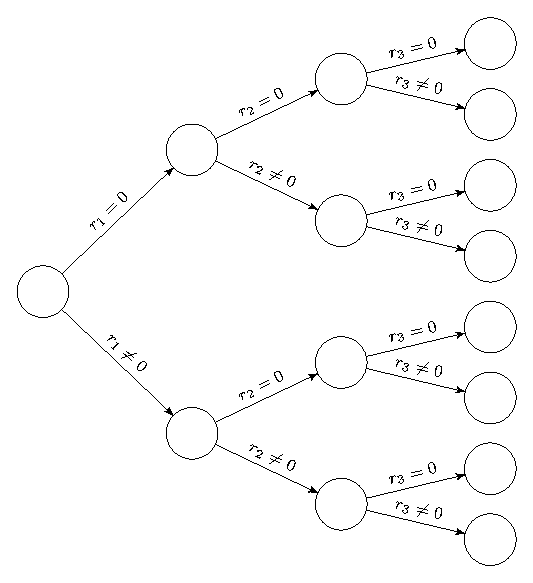
\includegraphics[width=.4\textwidth]{Figures/tree.eps}}
\caption{Na\"{\i}ve approach. Starting from the left, a each parameter $r_i$ has to be chosen either cell type-independent ($r_i=0$) or -specific ($r_i\neq 0$). Hence, the number of model candidates with grows exponentially with the number of parameters.}\label{fig:01}
\end{figure}

\subsection{Unbiased parameter estimation}

To estimate parameters $p$ for $n$ data points ${y_i}$, given values of the correspoding observation function observation $g(t_i,p)$, the negative two-fold log likelihood
\begin{equation}
-2\log \mathcal L(p) = \sum_{i=1}^n \frac{(y_i-g(t_i,p))^2}{\sigma_i^2} =: \chi^2\label{eq:lik}
\end{equation}
is optimized, resulting in the maximum likelihood estimate
\begin{equation}
\hat p = \text{arg}\min \left[ -2\log \mathcal L(p) \right] \:.
\end{equation}
Multi-start deterministic local optimization is often applied to ensure that $\hat p$ is in fact the global optimum.

\subsection{Regularization}
Regularization is often applied to incorporate prior knowledge or to improve numerics of parameter estimation.
Here, we persue a different strategy.
Regularization is used to assess the fold-change $\tilde r_i = 10^{r_i}$ of parameters between two cell types, i.e. $p_1 = \tilde r \cdot p_2$.
Thus, a constrained likelihood
\begin{equation}
-2\log \mathcal L_{L_k}(p,r) = -2\log \mathcal L(p) + \lambda \sum_i ||\log \tilde r_i||_k\label{eq:likreg}%\vspace*{-4pt}
\end{equation}
is implemented consisting of the likelihood (Eq.~\ref{eq:lik}) and a $L_k$ regularization term, weighted by $\lambda$.
The regularization term corresponds to a prior in a Bayesian framework:
For $k=0$ the $L_0$ prior is a delta distribution, for $k=1$ the $L_1$ prior is Laplacian function, and for $k=2$ the $L_2$ prior is a Gaussian function.\\
Different metrics $L_k$ show different properties.
$L_0$ would be ideal for our task due to its' direct penalization of the number of $r_i \neq 0$.
However, $L_0$ is not recommended because the associated optimization problem is known to be NP-hard.
In general, for $k<1$, the $L_k$ metric is non-convex which severly hampers parameter estimation.
On the other hand, both $L_0$ and $L_1$ induce sparsity and under some conditions they even give the same results on selection.
In contrast, $L_k$ for $k>1$ does not give sparse results, $L_2$ for instance is efficient but not sparse.
In that sense, the $L_1$ metric is unique, because it is the only one which combines both features, convexity and sparsity.
Therefore, we use $k=1$ in the following.\\
Due to local optima, the MLE (Eq.~\ref{eq:lik}) is obtained for individual cell types.

\begin{figure}[!tpb]%figure1
\centerline{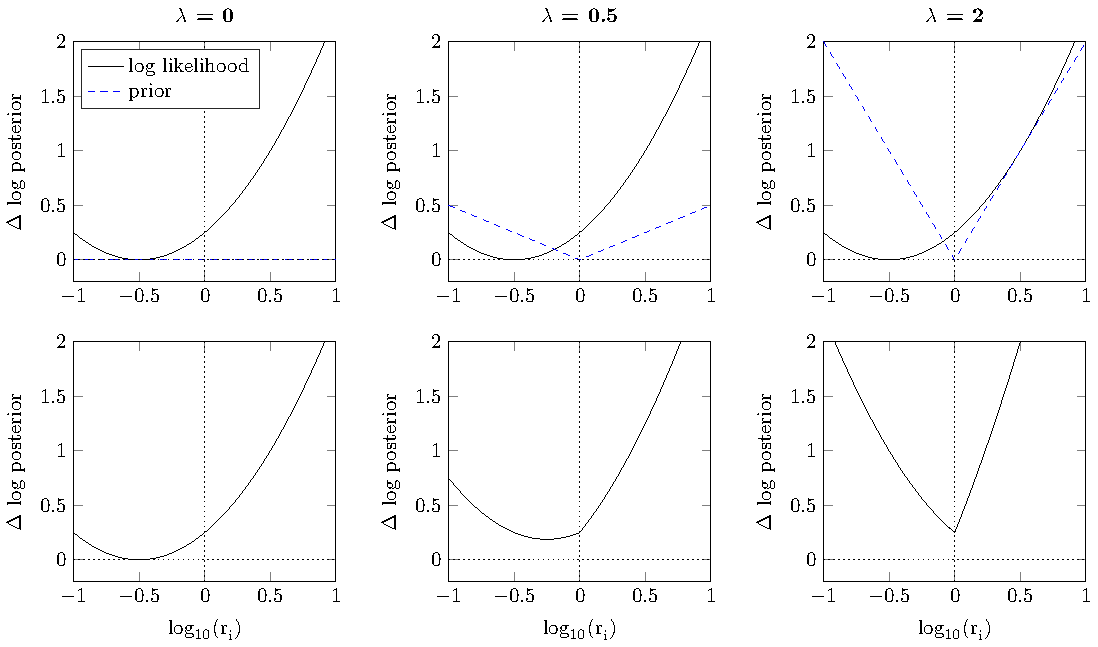
\includegraphics[width=235pt]{Figures/l1_cartoon_priorstrength.pdf}}
\caption{Exemplary log-likelihood. Regularization and constrained likelihood for different regularization weight $\lambda$.}\label{fig:02}
\end{figure}

\subsection{Regularized parameter estimation}
Optimization in context of partially observed stiff non-linear coupled ODE is non-trivial.
However, methods have been developed to efficiently solve this problem.
To augment the existing implementations with $L_1$ regularization, i.e. to minimize
\begin{equation}
	-2\log \mathcal L_{L_1}(p,r) = -2\log \mathcal L(p) + \lambda \sum_i |r_i|
\end{equation}
the following considerations are necessary.
Efficient optimization routines often exploit the quadratic form in (Eq.~\ref{eq:lik}).
For example, the implementation of a trust-region method \textit{lsqnonlin} in Matlab expects residuals
\begin{equation}
	\text{res}_i = \frac{y_i-g(t_i,p)}{\sigma_i}
\end{equation}
as input and implicitely converts these to a likelihood.
To implement optimization of the posterior (Eq.~\ref{eq:likreg}),
\begin{equation}
	\text{res}_i = \sqrt{\frac{|r_i|}{1/\lambda}}
\end{equation}
is appended to the residuals vector.
The associated sensitivites are given by
\begin{equation}
	\text{sres}_{ii} = \frac{\text{sgn}(r_i)}{\frac{2}{\lambda}\sqrt{\frac{|r_i|}{1/\lambda}}} \:.\label{eq:sres}
\end{equation}
Therefore, the gradient components
\begin{equation}
	g_i = 2 \: \text{res}_i \cdot \text{sres}_{ii} = \pm \lambda
\end{equation}
matches the theoretical value.
For $r_i = 0$, Eq.~\ref{eq:sres} is not defined.
In this case, the convergence criterion
\begin{equation}
	\begin{cases}
	\nabla_i \chi^2(\hat r_i) + \lambda \text{ sign}(\hat r_i) = 0, \:\:& |\hat r_i| > 0\\
	|\nabla_i \chi^2(\hat r_i)| \le \lambda, \:\:&\hat r_i = 0 \:.
	\end{cases}
	\label{eq:convcrit}
\end{equation}
is implemented by setting
\begin{equation}
	\begin{cases}
	\text{sres}_{ii}=0&|\nabla_i \chi^2(r_i)| > \lambda\\
	\text{sres}_{ij}=0\:\:\forall j, \:\:&|\nabla_i \chi^2(r_i)| \le \lambda \:.
	\end{cases}
	\label{eq:sresset}
\end{equation}
The rationale behind Eq.~\ref{eq:convcrit} is that the $L_1$ gradient either compensates the data gradient (first line), or that the $L_1$ gradient is stronger than the data gradient and keeps the estimate at its center $\hat r_i=0$ (second line).
During optimization, for a candidate $r_i=0$ this parameter-wise convergence criterion is checked at each optimization step.
While it is true, the derivative of each residual $j$ with respect to $r_i$ is set to zero, i.e. $\text{sres}_{ij}=0\:\:\forall j$.
If along optimization, the convergence criterion is not met anymore, only the ith $L_1$ contribution to the gradient is set to zero.
This enables $r_i$ that were zero to be released during optimization if there is strong evidence for it stemming from the data.

The $L_1$ metric has a discontinous derivative at zero.
In other words, the derivative changes for the optimizer unexpectedly as the sign of an $L_1$ regularized changes, also known as change of an orthant.
Hence, proposed optimization steps that change the orthant have to be avoided.
There are several methods that cope with this problem.
They have in common that they divide a proposed step into two:
first they step towards zero, then they move on.
Their major difference is the strategy how to step towards zero.
To keep the original behavior of trust-region based methods, we implemented the truncation of an optimization step such that the orthant is maintained.

\subsection{Profile likelihood}
The \emph{profile likelihood (PL)} constitutes a method to assess confidence intervals of parameters or predictions.
It does not rely on asymptotic assumptions and is therefore gives good results even in strongly non-linear settings.
The basic idea is to fix a certain model quantity, e.g. a parameter of interest, to a fixed value and re-optimize all other parameters. % Formula?
This re-optmizing procedure is iterated for different fixed values of the quantity of interest.
By comparing the decrease in goodness-of-fit confidence regions are calculated.

Here, we use \emph{PL} to check the parameter differences discovered by our algorithm.
Thus, the un-regularized \emph{PL} of fold-change parameter $r_i$ that is proposed using $L_1$ regularization is calculated.
If selection was successful, the \emph{PL} should not be compatible with 0.
This interpretation is equivalent to a likelihood ratio test between the null model $r_i=0$ and the alternative model $r_i \neq 0$.
However, the results are not expected to match exactly due to parameter dependencies that prevent $r_i=0$ for the regularized problem.

In addition, \emph{PL} can be used to investigate the uniqueness of the solution.
A non-uniquely selected parameter could be e.g. exchanged with another parameter that was not selected as difference.
Therefore, the \emph{PL} for each $r_i$ with estimate $\hat r_i=0$ is calculated.
This is equivalent to testing a model with 1 additional parameter ($r_i$) in comparison to parsimonious model ($r_i \equiv 0$).
If inside the CI of $r_i$, another parameter that was different to $0$ is now compatible with $0$, one cannot decide on the data which one is different.

Finally, regularized \emph{PL} of selected differences can pinpoint compensating effects.
Compensation manifests in piecewise flat regions in \emph{PL} though the regularization alone should already induce non-zero derivatives of \emph{PL}.
However, if a parameter change is compensated by adjusting another parameter, the regularizations can cancel out as well.
The \emph{PL} shape is then a clear indicator for compensation.

\begin{figure}[!tpb]%figure1
\centerline{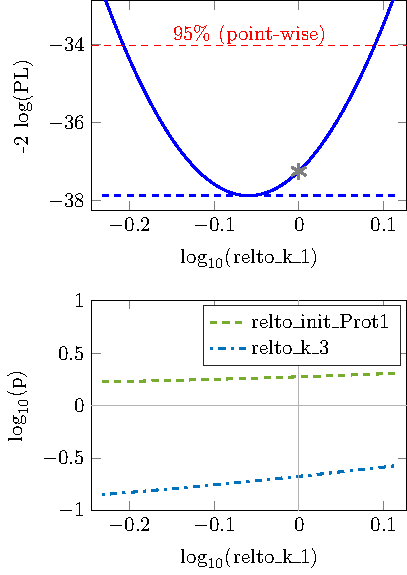
\includegraphics[width=110pt]{Figures/relto_k_1.pdf}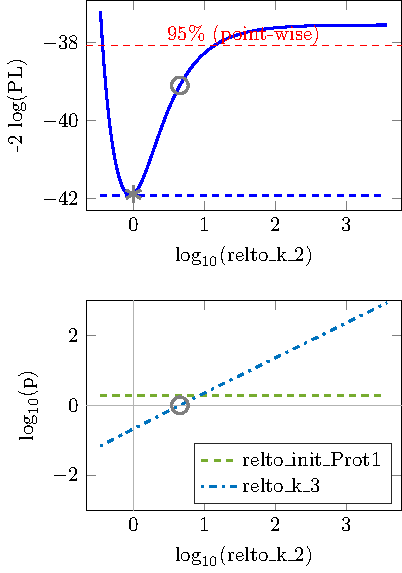
\includegraphics[width=110pt]{Figures/relto_k_2.pdf}}
\caption{Uniqueness and exchangeability.}\label{fig:01}
\end{figure}

\subsection{Regularization strength $\lambda$}
For generating model candidates, $\lambda$ is increased and the likelihood is re-optimized until mismatch between model and data is too large to reject the associated simplification.
This strategy is similar to the calculation of \emph{PL}, where a parameter of interest is fixed and the remaining parameters are re-estimated.
In both cases, likelihood-ratio statistics are employed to discover admissible regions.
For $L_1$ based feature selection, cross validation is often used to choose the final value for the regularization weight $\lambda$.
However, in nonlinear modeling, leaving data out could produce non-identifiablilites and the effect on the prediction error can be ambiguous.
Therefore, we decided to use an information theory based test criterion.
The most prominent methods are the likelihood ratio test (LRT), the Akaike information criterion (AIC), and the Bayesian information criterion (BIC).
The criteria are depicted by the vertical lines in Figure~4\vphantom{\ref{fig:04}} for an exemplary regularization path.
In certain settings these are equivalent: AIC resembles LRT for $\alpha = 15.6\%$.
With growing model size, $\alpha$ should be adjusted.
As this is not possible, we favor LRT over AIC.
BIC takes model size into account and is therefore equivalent to LRT with adjusted $\alpha$.
Because the selection criteria BIC and LRT hence comparable, we only use LRT in the following without loss of generality.\\
At the end, a good method should optimize specificity and sensitivity.
Thus, the result should as close as possible to the upper-left corner of the ROC curve.

\begin{figure}[!tpb]%figure1
\fboxsep=0pt\colorbox{gray}{\begin{minipage}[t]{235pt} \vbox to 100pt{\vfill\hbox to
235pt{\hfill\fontsize{24pt}{24pt}\selectfont FPO\hfill}\vfill}
\end{minipage}}
%\centerline{\includegraphics{fig01.eps}}
\caption{Regularization path. Show different selection criteria (LRT, AIC, BIC).}\label{fig:04}
\end{figure}

%Equation~(\ref{eq:01}) Text Text Text Text Text Text  Text Text
%Text Text Text Text Text Text Text Text Text Text Text Text Text.
%Figure~2\vphantom{\ref{fig:02}} shows that the above method  Text
%Text Text Text  Text Text Text Text Text Text  Text Text.
%\citealp{Boffelli03} might want to know about text text text text
%.....


\begin{methods}
\section{Approach}
% This section needs improvement. What are the exact steps to be performed for L1 analysis?
Given an overarching model that is able to describe two cell types with parameter vectors $p_1$ and $p_2$ for cell types 1 and 2, respectively.
Eq.~\ref{eq:likreg} is used to $L_1$ penalize the fold-change parameters $r$.
Then, $\lambda$ is scanned and the number of cell type specific parameters is observed.
For chosing the optimal $\lambda$, the un-regularized Eq.~\ref{eq:lik} is optimized, under the constraint that parameters with $r_i = 0$ are shared between both cell types.
The full model with all parameters specific for each cell type is then compared by the likelihood ratio test to each of the models that were selected using $L_1$ regularization.
Finally, the most parsimoneous model is defined as the smallest model that cannot be rejected by the likelihood ratio test.\\
Exemplary, we investigate uniqueness by \emph{PL}.
For giving a statistical assessment of the method it is unfeasible to perform this supervised uniqueness analysis for each iteration.
However when applied in practice results can be further improved by this manual analysis.
To mimic the manual inspection of the results, we implemented a heuristic that tests each $L_1$ parameter against zero from their order of deviation from zero.
If the likelihood did not increase by more than 1, the correction was accepted.
We show exemplarily for the application how the heuristic performs against a supervised manual inspection.
Further, plotting unobserved components for both cell types can enables validation design by discovering dynamics with a small prediction CI, which are different between the cell types.

%Text Text Text Text Text Text  Text Text Text Text Text Text Text
%Text Text Text Text Text Text Text Text.
%Figure~2\vphantom{\ref{fig:02}} shows that the above method  Text
%Text Text Text Text Text Text Text Text Text  Text Text.
%\citealp{Boffelli03} might want to know about text text text
%text\vspace*{1pt}
%
%\begin{itemize}
%\item for bulleted list, use itemize
%\item for bulleted list, use itemize
%\item for bulleted list, use itemize\vspace*{1pt}
%\end{itemize}
%
%Text Text Text Text Text Text  Text Text Text Text Text Text Text
%Text Text Text Text Text Text Text Text.
%Figure~2\vphantom{\ref{fig:02}} shows that the above method Text
%Text Text Text Text Text Text Text Text Text Text Text.
%\citealp{Boffelli03} might want to know about text text text text
%Text Text Text Text Text Text  Text Text Text Text Text Text Text
%Text Text Text Text Text Text Text Text.
%
%Text Text Text Text Text Text  Text Text Text Text Text Text Text
%Text Text  Text Text Text Text Text Text\vadjust{\newpage}.
%Figure~2\vphantom{\ref{fig:02}} shows that the above method  Text
%Text Text Text  Text Text Text Text Text Text  Text Text.
%\citealp{Boffelli03} might want to know about text text text text
%
%
%\subsection{This is subheading}
%
%Text Text Text Text Text Text Text Text Text Text Text Text Text
%Text Text  Text Text Text Text Text Text.
%Figure~2\vphantom{\ref{fig:02}} shows that the above method  Text
%Text Text Text Text Text Text Text Text Text  Text Text.
%\citealp{Boffelli03} might want to know about  text text text text
%Text Text Text Text Text Text  Text Text Text Text Text Text Text
%Text Text  Text Text Text Text Text Text.
%
%
%\subsubsection{This is subsubheading}
%
%Text Text Text  Text Text Text Text Text Text  Text Text.
%\citealp{Boffelli03} might want to know about  text text text text
%Text Text Text Text Text Text Text Text Text Text Text Text Text
%Text Text  Text Text Text Text Text Text.
%Figure~2\vphantom{\ref{fig:02}} shows that the above method  Text
%Text Text Text  Text Text Text Text Text Text  Text Text.
%\citealp{Boffelli03} might want to know about  text text text text
%
%\enlargethispage{6pt}
%
%
%Text Text Text Text Text Text  Text Text Text Text Text Text Text
%Text Text  Text Text Text Text Text Text.
%Figure~2\vphantom{\ref{fig:02}} shows that the above method  Text
%Text Text Text  Text Text Text Text Text Text  Text Text.
%\citealp{Boffelli03} might want to know about  text text text text


\end{methods}

%\begin{figure}[!tpb]%figure2
%%\centerline{\includegraphics{fig02.eps}}
%\caption{Caption, caption.}\label{fig:02}
%\end{figure}

%Text Text Text Text Text Text  Text Text Text Text Text Text Text
%Text Text  Text Text Text Text Text Text.
%Figure~2\vphantom{\ref{fig:02}} shows that the above method  Text
%Text Text Text  Text Text Text Text Text Text  Text Text.
%\citealp{Boffelli03} might want to know about  text text text text\vspace{10pt}

\section{Application}
\subsection{Model description}
In the following, we use the first model of the \emph{DREAM6 (Dialogue for Reverse Engineering Assessment and Methods)} challenge as benchmark for our approach.
The in-silico model mimics a gene-regulatory network and is based on realistic assumptions.
It was used in 2011 to evaluate the performance of experimental design strategies to optimize parameters and predictions.
The model incorporates transcription and translation dynamics of 6 genes.
Therefore, the dynamic variables represent 6 mRNAs, as well as the 6 associated proteins with known intial concentrations.
Positive and negative regulation between genes is possible.
Taken together, the model consits of 29 parameters.
13 are associated with generation and degradation of molecules:
1 protein degradation rate which is shared among all proteins; 
6 ribosomal strengths determining the production rate of mRNAs;
6 protein production strengths which define how strong mRNA presence induces protein synthesis;
The remaining 16 parameters define the interaction of genes by Hill kinetics, thus 8 $K_D$ values and 8 Hill coefficients are assumed.

DREAM6 M1 was simulated with gold-standard parameters that were made publicly available after completion of the challenge.
We now use this gold-standard as cell type 1.
When complete data is provided, i.e. all observables measured at all possible experimental condidtions, all parameters are identifiable, except for one Hill coefficient which is only restricted to lower values.
Thus, we conclude that determining parameter differences between cell types is possible in principle.
Next, we assumed 1/3 of all parameters to be cell type-specific.
We therefore randomly simulated fold-changes of $[2~5~10]$ for non-Hill parameters in both directions.
For Hill coefficients, fold changes of $1/2$ and $1/4$ were assumed, under the constraint that the modified values stay inside the interval $[1~4]$.
This assumption for the range is biologically reasonable as the number of binding sites on a molecule is thereby considered.
Taken together, the number of possible models is $2^{29}>5\cdot10^8$.

In the original DREAM6 challenge, there were basically two observation types available:
(1) mRNA measurements for all mRNAs with 21 data-points each, or (2) protein measurements for 2 proteins which had to be specified, each with 41 data-points.
The observation function was the identity, i.e. the molecular compounds were observed directly without scaling or offset parameters.
The error model was consisted of an absolute term as well as a relative term with given contributions.
% If a trajectory was near zero, negative data points may occur which were then set to zero to avoid negative concentrations.
In addition to wildtype data, there was the option of performing 3 possible perturbations per each node $i$ out of 6 nodes:
\begin{enumerate}
\item knock-out ($\text{mRNA\_pro}_i=\text{Prot\_pro}_i=0$)
\item knock-down ($\text{mRNA\_deg}_i\rightarrow 5\cdot \text{mRNA\_deg}_i$)
\item over-expression ($\text{mRNA\_pro}_i \rightarrow 2\cdot \text{mRNA\_pro}_i$)
\end{enumerate}
In total, this results in 18 possible experimental conditions.
To have a reference for perturbations we decided during the original challenge to purchase all wildtype data, i.e. mRNA and protein data for all observables.
After acquiring wildtype data the remaining budget was sufficient for around 9 additional data-sets, which had to be selected from $331$ possibilities.
To allow some variability in the number of experiments, we randomly (50\%) selected for each of the 18 conditions whether the conditions was included in the observation.
To mimic the partial observation which was one task of the DREAM6 challenge, we chose random whether mRNA (1/3) or proteins (2/3) were observed.
Given the latter, 2 out of 6 proteins were randomly selected.
We chose the same experimental conditions and observables for both cell types.

After implementing the fold-changes between cell types, as well as perturbations and observerations we used a $L_1$ regularization for all fold-change parameters and scanned along $\lambda$ for variable selection.
For selection of $\lambda$ we used the unpenalized solution.
Thus, we could ensure an unbiased estimate of the fold-change parameters.

\subsection{Performance assessment}
The procedure of selecting fold-changes and observations was iterated $N=500$ times, yielding a random sample of $2^{29} \cdot 331 > 10^{11}$ possibilities.
The performance is summarizes in Figure~5\vphantom{\ref{fig:05}}.
The black line depicts the average ROC curve, the shading gives the standard deviation over all $N=500$ iterations.
The blue dots show the selected parsimonious model selected by the likelihood-ratio test.
Usually, for a given ROC curve the selection criterion is chosen to maximize both sensitivity and specificity simulateously, which is the point most up-left on the ROC curve.
Because the blue dots appear centered around this `kink', we consider our selection criterion appropriate.

We further evaluated the performance of our $L_1$ fold-change detection routine for different parameter types.
The results are summarizes in Table~1\vphantom{\ref{Tab:01}}.
The protein degradation rate which is shared among all proteins is detected in 100\% as difference when there was a difference simulated.
On the other hand, this parameter also had the highest false positive rate with round 44\%.
A possible explanation is given by the fact that our method is data driven and hence differences are more likely to be detected in points of the network with more data available.
This is the case for the protein degradation rate because it influences all proteins in the network.
The individual protein production and ribosomal strengths have a decent false positive rate between 20\% and 30\% and a true positive rate of over 80\%.
In contrast, the Hill regulation parameters ($K_D$ and Hill coefficient) are detected less frequently as difference.
Probably, this is due to identifiability issues as those parameters were already the most difficult ones to estimate in the original DREAM6 challenge.
The underlying reason is that the concentration range around $K_D$ has to be sampled for a reliable estimation which cannot be ensured without proper experimental design.

% Performance for different fold-changes\\ % Wie bewertet man das am besten? Braeuchte man evtl. Unsicherheitsabschaetzungen ...
Performance for different ratio of protein vs mRNA measurement

\begin{figure}[!tpb]%figure1
\centerline{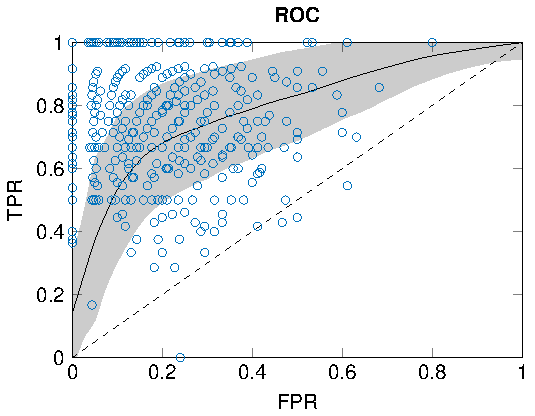
\includegraphics[width=235pt]{Figures/ROC.pdf}}
\caption{ROC curve displaying the performance of the implementation on DREAM6 M1. No experimental design was performed. $N = 500$. Black line is average ROC curve. Shading is standard deviation. Blue circles denote selected model for all iterations. Because the dots appear on average near the maximum of sensitivity and specificity (upper left corner), the selection criterion is appropriate.}\label{fig:05}
\end{figure}

\subsection{Manual inspection}
In the following, we select one representative iteration out of the $N=500$ given by a minimal deviation of its ROC curve to the average ROC curve.
For the automatic model selection shown in the previous section, $\lambda$ was scanned around the selected value.
Now, we use a higher grid density for $\lambda$ to visualize the regularization path in Figure X.
Next, we calculate \emph{PL} for each regularized parameter to check for compensating effects.
This facilitates the removal of YY additional parameters.
Finally, we checked by calculating \emph{PL} of the unregularized fold-change parameters whether the results are not compatible with zero.
This was the case.
In comparison to the automatically detected parameter differences, the result of the manual inspection decreased the FPR from XX\% to YY\% and increased the TPR from XX\% to YY\%.
We therefore advise manual inspection in a real world application to maximize the performance of the method.

\begin{table}[!t]
\processtable{Performance of algorithm on DREAM6 M1\label{Tab:01}} {\begin{tabular}{@{}llll@{}}\toprule Parameter class &
N & FPR & TPR\\\midrule
Protein degradation rate & 57 & 0.4409 & 1.0000\\
Protein production strength & 309 & 0.2927 & 0.8350\\
Ribosomal strength & 282 & 0.2071 & 0.8191\\
$K_D$ value & 418 & 0.1560 & 0.6842\\
Hill coefficient & 396 & 0.2164 & 0.6843\\\hline
All & 1462 & 0.2209 & 0.7544\\\botrule
\end{tabular}}{Protein degradation rate is shared among all and hence often diagnosed as difference. Strengths are well-balanced for FPR and TPR. $K_D$ and Hill coefficients are difficult to detect because concentration range around $K_D$ has to be covered to see effect on dynamics. 500 iterations were computed. Each iteration ($L_1$ regularized scan; unregularized fits) took 28.8 min on average on an Intel Xeon E5-1620 3.60Ghz desktop computer.}
\end{table}


%Text Text Text Text Text Text  Text Text Text Text Text Text Text
%Text Text  Text Text Text Text Text Text.
%Figure~2\vphantom{\ref{fig:02}} shows that the above method  Text
%Text Text Text  Text Text Text Text Text Text  Text Text.
%\citealp{Boffelli03} might want to know about  text text text text
%
%
%Table~\ref{Tab:01} shows that Text Text Text Text Text  Text Text
%Text Text Text Text. Figure~2\vphantom{\ref{fig:02}} shows that
%the above method Text Text. Text Text Text  Text Text Text Text
%Text Text. Figure~2\vphantom{\ref{fig:02}} shows that the above
%method Text Text. Text Text Text  Text Text Text Text Text Text.
%Figure~2\vphantom{\ref{fig:02}} shows that the above method Text
%Text.









%%%%%%%%%%%%%%%%%%%%%%%%%%%%%%%%%%%%%%%%%%%%%%%%%%%%%%%%%%%%%%%%%%%%%%%%%%%%%%%%%%%%%
%
%     please remove the " % " symbol from \centerline{\includegraphics{fig01.eps}}
%     as it may ignore the figures.
%
%%%%%%%%%%%%%%%%%%%%%%%%%%%%%%%%%%%%%%%%%%%%%%%%%%%%%%%%%%%%%%%%%%%%%%%%%%%%%%%%%%%%%%






\section{Discussion}

Differences to linear setting.\\
Parameters are not necessarily monotoneous.\\
Exchangeability\\
Compensation $\rightarrow$ only subgroup necessary to be different\\
Scanning $\lambda$ not necessarily globaly optimal.\\
Regularization might induce additional local optima that could be globally optimal.\\
Numerics tough in the vicinity of 0.\\
\begin{equation}
	H_{ij} \approx \text{sres}_i \cdot \text{sres}_j = \frac{\text{sgn}(r_i)}{\frac{2}{\lambda}\sqrt{\frac{|r_i|}{1/\lambda}}} \cdot \frac{\text{sgn}(r_j)}{\frac{2}{\lambda}\sqrt{\frac{|r_j|}{1/\lambda}}}
\end{equation}
\begin{equation}
	\lim_{r_i \rightarrow 0} H_{ij} = \lim_{r_j \rightarrow 0} H_{ij} = \pm \infty
\end{equation}
L1.x does not help either (not sparse)\\
Combos do not help either (in vicinity of 0, $L_1$ dominates anyway)\\
Check cross-validation\\
Check shrinkage\\
L2 might be an option --> Daniel\\ \\
DREAM specific discussion\\
Lack of observation function\\
No differences in initials\\
Non-identifiability may decrease TPR\\
Hills hard to detect (range is important)\\
Experimental design principles were not applied, which were the task in the original DREAM6 challenge. Therefore, one cannot expect perfect detection of cell type specific parameters due to identifiability issues.\\
Method data driven

%(Table~\ref{Tab:01}) Text Text Text Text Text Text  Text Text Text
%Text Text Text Text Text Text  Text Text Text Text Text Text.
%Figure~2\vphantom{\ref{fig:02}} shows that the above method  Text
%Text Text Text  Text Text Text Text Text Text  Text Text.
%\citealp{Boffelli03} might want to know about  text text text text
%
%\begin{enumerate}
%\item this is item, use enumerate
%\item this is item, use enumerate
%\item this is item, use enumerate
%\end{enumerate}
%
%Text Text Text Text Text Text Text Text Text Text Text Text Text
%Text Text Text Text Text Text Text Text.
%Figure~2\vphantom{\ref{fig:02}} shows\vadjust{\pagebreak} that the
%above method  Text Text Text Text Text Text Text Text Text Text
%
%
%Text Text Text Text Text Text  Text Text Text Text Text Text Text
%Text Text  Text Text Text Text Text Text.
%Figure~2\vphantom{\ref{fig:02}} shows that the above method  Text
%Text Text Text\vspace*{-10pt}


\section*{Acknowledgements}

Text Text Text Text Text Text  Text Text.  \citealp{Boffelli03} might want to know about  text
text text text\vspace*{-12pt}

\section*{Funding}

This work has been supported by the... Text Text  Text Text.\vspace*{-12pt}

\bibliographystyle{natbib}
%\bibliographystyle{achemnat}
%\bibliographystyle{plainnat}
%\bibliographystyle{abbrv}
% \bibliographystyle{bioinformatics}

% \bibliographystyle{plain}

\bibliography{document}

\end{document}
